\tikzstyle{area} = [rectangle,draw,minimum height=3cm,minimum width=2cm]
\tikzstyle{assembly} = [rectangle,draw,minimum height=0.75cm,minimum width=0.5cm]
\tikzstyle{every node}=[font=\LARGE]
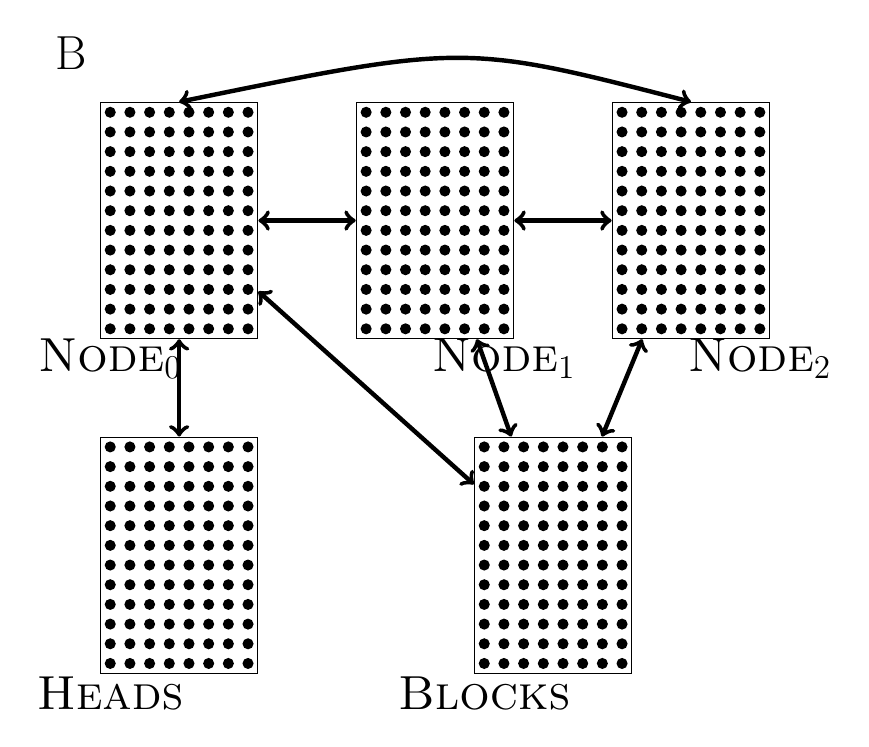
\begin{tikzpicture}[x=0.25cm,y=0.25cm]
    \begin{scope}[xshift=1.5cm]
	\node[area] (B) at (3.5,5.5) {};
	\node at (0,-1.5) {\textsc{Blocks}};
	\foreach \x in {0,...,7}
	\foreach \y in {0,...,11}
	{\fill (\x,\y) circle (2pt);}
	\end{scope}
	\begin{scope}[xshift=-3.25cm,yshift=4.25cm]
	\node[area] (N1) at (3.5,5.5) {};
	\node at (0,-1.5) {\mbox{\textsc{Node}$_0$}};
	\foreach \x in {0,...,7}
	\foreach \y in {0,...,11}
	{\fill (\x,\y) circle (2pt);}
	\draw[<->,ultra thick] (B) -- (N1);
	\end{scope}
	\begin{scope}[xshift=0cm,yshift=4.25cm]
	\node[area] (N2) at (3.5,5.5) {};
	\node at (7,-1.5) {\mbox{\textsc{Node}$_1$}};
	\foreach \x in {0,...,7}
	\foreach \y in {0,...,11}
	{\fill (\x,\y) circle (2pt);}
	\draw[<->,ultra thick] (B) -- (N2);
	\draw[<->,ultra thick] (N1) -- (N2);
	\end{scope}
	\begin{scope}[xshift=3.25cm,yshift=4.25cm]
	\node[area] (N3) at (3.5,5.5) {};
	\node at (7,-1.5) {\mbox{\textsc{Node}$_2$}};
	\foreach \x in {0,...,7}
	\foreach \y in {0,...,11}
	{\fill (\x,\y) circle (2pt);}
	\draw[<->,ultra thick] (B) -- (N3);
	\draw[<->,ultra thick] (N2) -- (N3);
	\draw[bend right,<->,ultra thick] (N1.north) .. controls (-8,14.5) .. (N3.north);
	\end{scope}
	\begin{scope}[xshift=-3.25cm,yshift=0cm]
	\node[area] (H) at (3.5,5.5) {};
	\node at (0,-1.5) {\textsc{Heads}};
	\foreach \x in {0,...,7}
	\foreach \y in {0,...,11}
	{\fill (\x,\y) circle (2pt);}
	\draw[<->,ultra thick] (H) -- (N1);
	\end{scope}
	\node at (-15,31) {\LARGE B};
\end{tikzpicture}